\section{Ziel}
Ziel des Versuches war es die Zusammensetzung eines 3x3x3-Würfels in einer seiner Ebene zu bestimmen, wobei die einzelnen Teilwürfel aus unterschiedlichen Metallen besteht. 

\section{Theorie}
\subsection{Tomographie}
Die Tomographie ist ein Bild-gebendes Verfahren, welches viel Anwendung in der heutigen Medizin findet. Besonders die so genannte Computertomographie, kurz CT, ist weit 
verbreitet.
Durch dieses Verfahren werden Querschnitte erzeugt und durch die Untersuchung mehrerer Schichten kann so ein 3 Dimesnionales Bild generiert werden.

\noindent
Im Allgemeinen wird für die Tomographie $\gamma$-Strahlung benutzt. Durch die unterschiedlichen Absorptionskoeffizienten und durch die Bestrahlung des Targets aus 
verschiedenen Winkeln kann ein Bild erzeugt werden.

\subsection{Wechselwirkung von Materie mit Gamma-Strahlung}
Die Quelle der $\gamma$-Strahlung ist im Versuch der Zerfall eines radioaktiven Isotops. In diesem zerfällt
der Kern unter Aussendung eines $\gamma$-Quants in ein energetisch günstigeren Zustand. Dadurch ist das 
Spektrum der $\gamma$-Strahlung diskret.

\noindent
$\gamma$-Strahlung wechselt wirkt hauptsächlich in 3 Art und Weisen mit Materie. 
Diese sind der Photoeffekt, die Compton-Streuung, sowie die Paarerzeugung.
\begin{enumerate}
  \item \textbf{Photo-Effekt}:
  Beim Photoeffekt wird ein Photon vollständig von einem gebundenen Elektron absorbiert so, dass dieses aus seiner Bindung herausgelöst wird. 
  Dafür muss die Energie des $\gamma$-Quants ($E_\gamma = \symup{h}f$) mindestens die Bindungsenergie $E_B$ des Elektrons an den Kern betragen. Die
  kinetische Energie des Elektrons lässt sich somit bestimmen zu 
  \begin{equation}
    E_{\symup{e}} = E_\gamma - E_{\symup{B}}
    \label{eqn:1}
  \end{equation}

  \noindent
  Der Wirkungsquerschnitt $\sigma$ ist $\propto Z^5E_\gamma^{-3,5}$, daher dominiert im Allgemeinen 
  der Photoeffekt bei Energien <100keV und bei Kernen mit einer hohen Ladungszahl $Z$.

  \item \textbf{Comptonstreuung}:
  Bei der Comptonstreuung,  auch inelastische Streuung genannt, trifft ein Photon auf ein quasi-freies Elektron. 
  Das Photon gibt dabei einen Teil seiner Energie $\delta \symup{E}$
  ab, sodass die Wellenlänge um $\delta\lambda = \lambda' - \lambda $ verändert wird.
  Wichtig für den Energieübertrag ist dabei der Winkel in dem das Photon auf das Elektron trifft. Der 
  Energieübertrag wird maximal für $180°$. Zudem werden beide Teilchen von ihrer ursprünglichen Bahn abgelenkt
, sodass eine Streuung statt findet.

\noindent
Die Comptonstreuung dominiert für Energien im Bereicht von 100keV - 1MeV.


  \item \textbf{Paarerzeugung}:
  Bei der Paarerzeugung zerfällt ein Photon in einem Coulombfeld eines Teilchens in ein Teilchen-Antiteilchen Paar.
  Die benötigte Mindestenergie für ein $\gamma$-Quant ist gesetzt durch die doppelte Masse des Elektrons (da diese
  identisch mit der Masse des Positrons ist), da dieses Pärchen das leichteste ist, in welches es Zerfall kann.
  Somit ist die Mindestenergie gegeben durch 
  \begin{equation}
    E_\gamma =  2 \symup{m}_e \symup{c}^2 \, .
    \label{eqn:3}
  \end{equation}
\end{enumerate}

\noindent
Da in diesem Versuch lediglich Energien bis $E_{\gamma} = 662$ keV erreicht werden, spielt der Effekt der Paarerzeugung keine wichtige Rolle. 


\subsection{Radioaktiverzerfall}
Wie bereits oben beschrieben wird als $\gamma$-Strahlungsquelle ein radioaktiver Zerfall benutzt. Es kann entweder ein $^{60} Co$ oder $^{137} Cs$-Strahler genutzt werden.
Da im Versuch eine $^{137} Cs$ Quelle verwendet wurde wird expemplarisch nur auf diesen Zerfall eingegangen.

\noindent
Im dominierenden Zerfallskanal, mit einer Zerfallswahrscheinlichkeit von 94,4\%, zerfällt $^{137} Cs$ in einen angeregten Zustand vom Barium $^{137m} Ba$. Welches dann
unter Emission eines Photons in den Grundzustand vom Barium $^{137} Ba$ übergeht. Bei diesem Zerfall eintsteht eine mittlere Photonenenergie von $E_{\gamma} = 661,7$ keV \cite{Zerfall}.
Der Zerfall ist ebenfalls in Abbildung (\ref{fig:zer}) dargestellt.


\begin{figure}
  \centering
  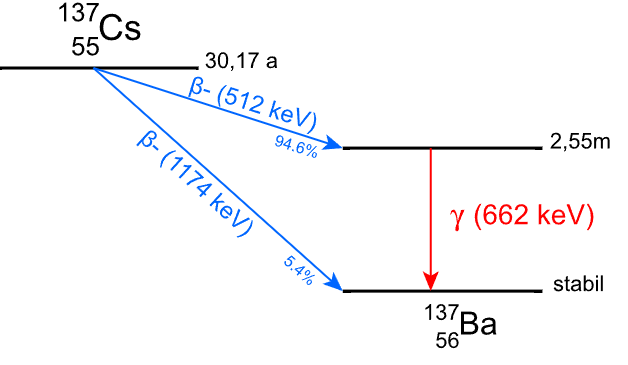
\includegraphics[width=0.75\textwidth]{zerfall.png}
  \caption{Zerfall eines $^{137} Cs$ Atoms \cite{Zerfall}}
  \label{fig:zer}
\end{figure}


\subsection{Abschwächung}
Wenn Strahlung Materie durchdringt wechselwirkt sie mit dieser. Dardurch verliert sie Energie und es wird von einer Abschwächung gesprochen.
Im Allgemeinen kann die Intensitätsveränderung beschrieben werden durch 

\begin{equation}
  N = I_0 exp \left(- \sum_i \mu_i d_i \right) \, .
  \label{eqn:exp}
\end{equation}

Dabei sind $\mu_i$ die Absorptionskoeffizienten, $I_0$ die Eingansintensität und $d_i$ die Länge der Strecke, in welcher die Strahlung wechselwirkt. Dies 
lässt sich nun umstellen zu 

\begin{equation}
  \sum_i \mu_i d_i = log \left( \frac{I_0}{N_j}  \right) = I_i \, .
  \label{eqn:log}
\end{equation}

Hierbei steht $N_j$ für die jeweils gemessenen Ausgangsintensitäten. Aus diesem Zusammenhang kann ein LGS (kurz für Lineares Gleichungssystem) aufgestellt werden.

\noindent
Da im Versuch ein 3x3-Würfel tomographisch untersucht wurde, kann eine Matrix $\underline{\underline{A}}$ in dem Zusammenhang 

\begin{equation}
  \underline{\underline{A}} \vec{\mu} = \vec{I} 
  \label{eqn:matrix}
\end{equation}

aufgestellt werden. Das LGS wird bewusst überbestimmt aufgestellt um eine hohe (Mess-)Fehleranfälligkeit zu senken, sodass die Matix (passend zu den Strahlengängen in der
\autoref{fig:projektion}) aussieht wie in \autoref{fig:matrix} dargestellt ist.

\begin{figure}[H]
	\centering
	\begin{subfigure}[b]{0.45\textwidth}
		\centering
		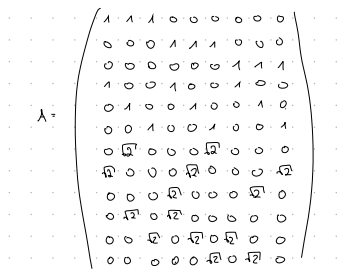
\includegraphics[width=4.5cm]{matrix.png}
		\caption{Matrix A}
    \label{fig:matrix}
	\end{subfigure}
	~
	\begin{subfigure}[b]{0.45\textwidth}
		\centering
		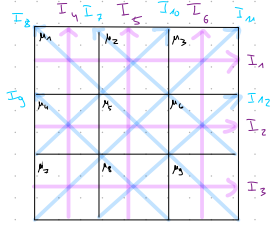
\includegraphics[width=4.5cm]{projektion.png}
		\caption{Schematische Darstellung der Strahlengänge durch den Würfel}
    \label{fig:projektion}
	\end{subfigure}
\end{figure}

